%%%%%%%%%%%%%%%%%%%%%%%%%%%%%%%%%%%%%%%%%%%%%%%%%%%%%%%%%%%
%                                                         %
% CHAPTER 03:                                             %
% The 2-electrons system                                  %
%                                                         %
% This file is part of a BSc Thesis Project. See the      %
% LICENSE file for more information about licensing.      %
%                                                         %
% Author:     Matteo Seclì <secli.matteo@gmail.com>       %
% A.Y.:       2014/2015                                   %
% URL:        https://github.com/matteosecli/QMC          %
%                                                         %
%%%%%%%%%%%%%%%%%%%%%%%%%%%%%%%%%%%%%%%%%%%%%%%%%%%%%%%%%%%

\graphicspath{{Mainmatter/figures/PNG/}{Mainmatter/figures/PDF/}{Mainmatter/figures/}}

\chapter{The 2-electrons system}

\section{The unperturbed system}
\label{sec:2e_unp}

\begin{figure}[H]
	\centering
	\definecolor{myblue}{rgb}{0,0.447,0.741}	
	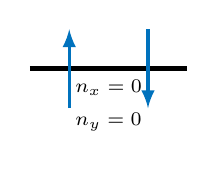
\begin{tikzpicture}
		\tikzset{>=latex}
		\draw [ultra thick] (-1,0) -- (1,0) node[midway,below,align=center] {\scriptsize $n_x=0$ \\ \scriptsize $n_y=0$};
		\draw [very thick, myblue, ->] (-0.5,-0.5) -- (-0.5,0.5);
		\draw [very thick, myblue, ->] (0.5,0.5) -- (0.5,-0.5);
	\end{tikzpicture}
	\caption{The 2-electrons system configuration.}
	\label{fig:sketch_2e}
\end{figure}

We will first consider the unperturbed system (without the electron-electron repulsion) with $\omega = 1$, that has Hamiltonian
\begin{equation}
	\hat{H}_0 = 
	\sum_{i=1}^{N} \left( -\frac{1}{2}\nabla_i^2 + \frac{1}{2}\omega^2r_i^2 \right),
\end{equation}
with $N=2$ and in two dimensions. For a single electron in a two-dimensional (isotropic) harmonic oscillator, the energy is $E_s = \hbar\omega(n_x + n_y + 1)$, where $n_x$ and $n_y$ are the quantum numbers for the $x$ and $y$ dimensions. The ground state (see Figure \ref{fig:sketch_2e}) is obtained for $(n_x,n_y) = (0,0)$ which gives $E_s = \SI{1}{\atomicunit}$. Since we have two particles, the ground state energy of our system is in total
\begin{equation*}
	E_{\text{gs}} = \SI{2}{\atomicunit}.
\end{equation*}
In general, for $\omega \neq 1$, the energy will just be $E_{\text{gs}} = 2\omega$.

Now, we have to choose a trial wave-function. For a single electron, the exact wave-function of the ground state is
\begin{equation}
	\phi_{n_x,n_y}(x, y) = A H_{n_x}(\sqrt{\omega}x)H_{n_y}(\sqrt{\omega}y)\exp\left(-\omega\left(x^2 + y^2\right)/2\right),
	\label{eq:phi_qnums}
\end{equation}
being $A$ a normalization constant and $H_n$ is the (physical) Hermite polynomial of order $n$. Since the 0-th order Hermite polynomials are just $1$ and the two-particles wave-function can be seen as a product of the single-particle wave-functions, our total wave-function will just be
\begin{equation}
	\phi(\vec{r}_1,\vec{r}_2) = C \exp\left(-\omega\left(r_1^2 + r_2^2\right)/2\right).
	\label{eq:two_part_noint_solution}
\end{equation}
Adding a variational parameter $\alpha$ and forgetting about the normalization constant $C$, we obtain our trial wave-function for this case:
\begin{equation}
	\psi_T(\vec{r}_1,\vec{r}_2) = \exp\left(-\alpha\omega\left(r_1^2 + r_2^2\right)/2\right).
\end{equation}
Note that, since the correct solution of this problem is equation (\ref{eq:two_part_noint_solution}), we expect to obtain a variational energy \emph{exactly} equal to 2 for $\alpha = 1$.

\begin{figure}[H]
	\centering
	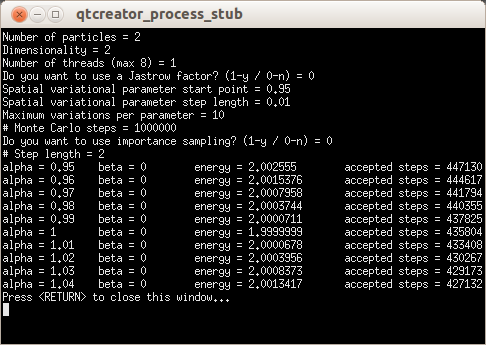
\includegraphics[width=0.45\textwidth]{two-part-non-int}
	\caption{The program running for a two-electron system without repulsion.}
	\label{fig:run_window_2e_no_rep}
\end{figure}

The electron-electron repulsion can be simply turned off by commenting out the line
\begin{lstlisting}[language=cpp]
	MySystem.add_potential(new eRepulsion(gP));
\end{lstlisting}
in the code. Running the program in Qt Creator shows the window in Figure \ref{fig:run_window_2e_no_rep}, where some parameters can be specified before the actual calculation begins.

Just using a finer step for $\alpha$, we obtain the energy graph shown in Figure \ref{fig:2e_no_rep}.
\begin{figure}[h]%[H]
	\centering
	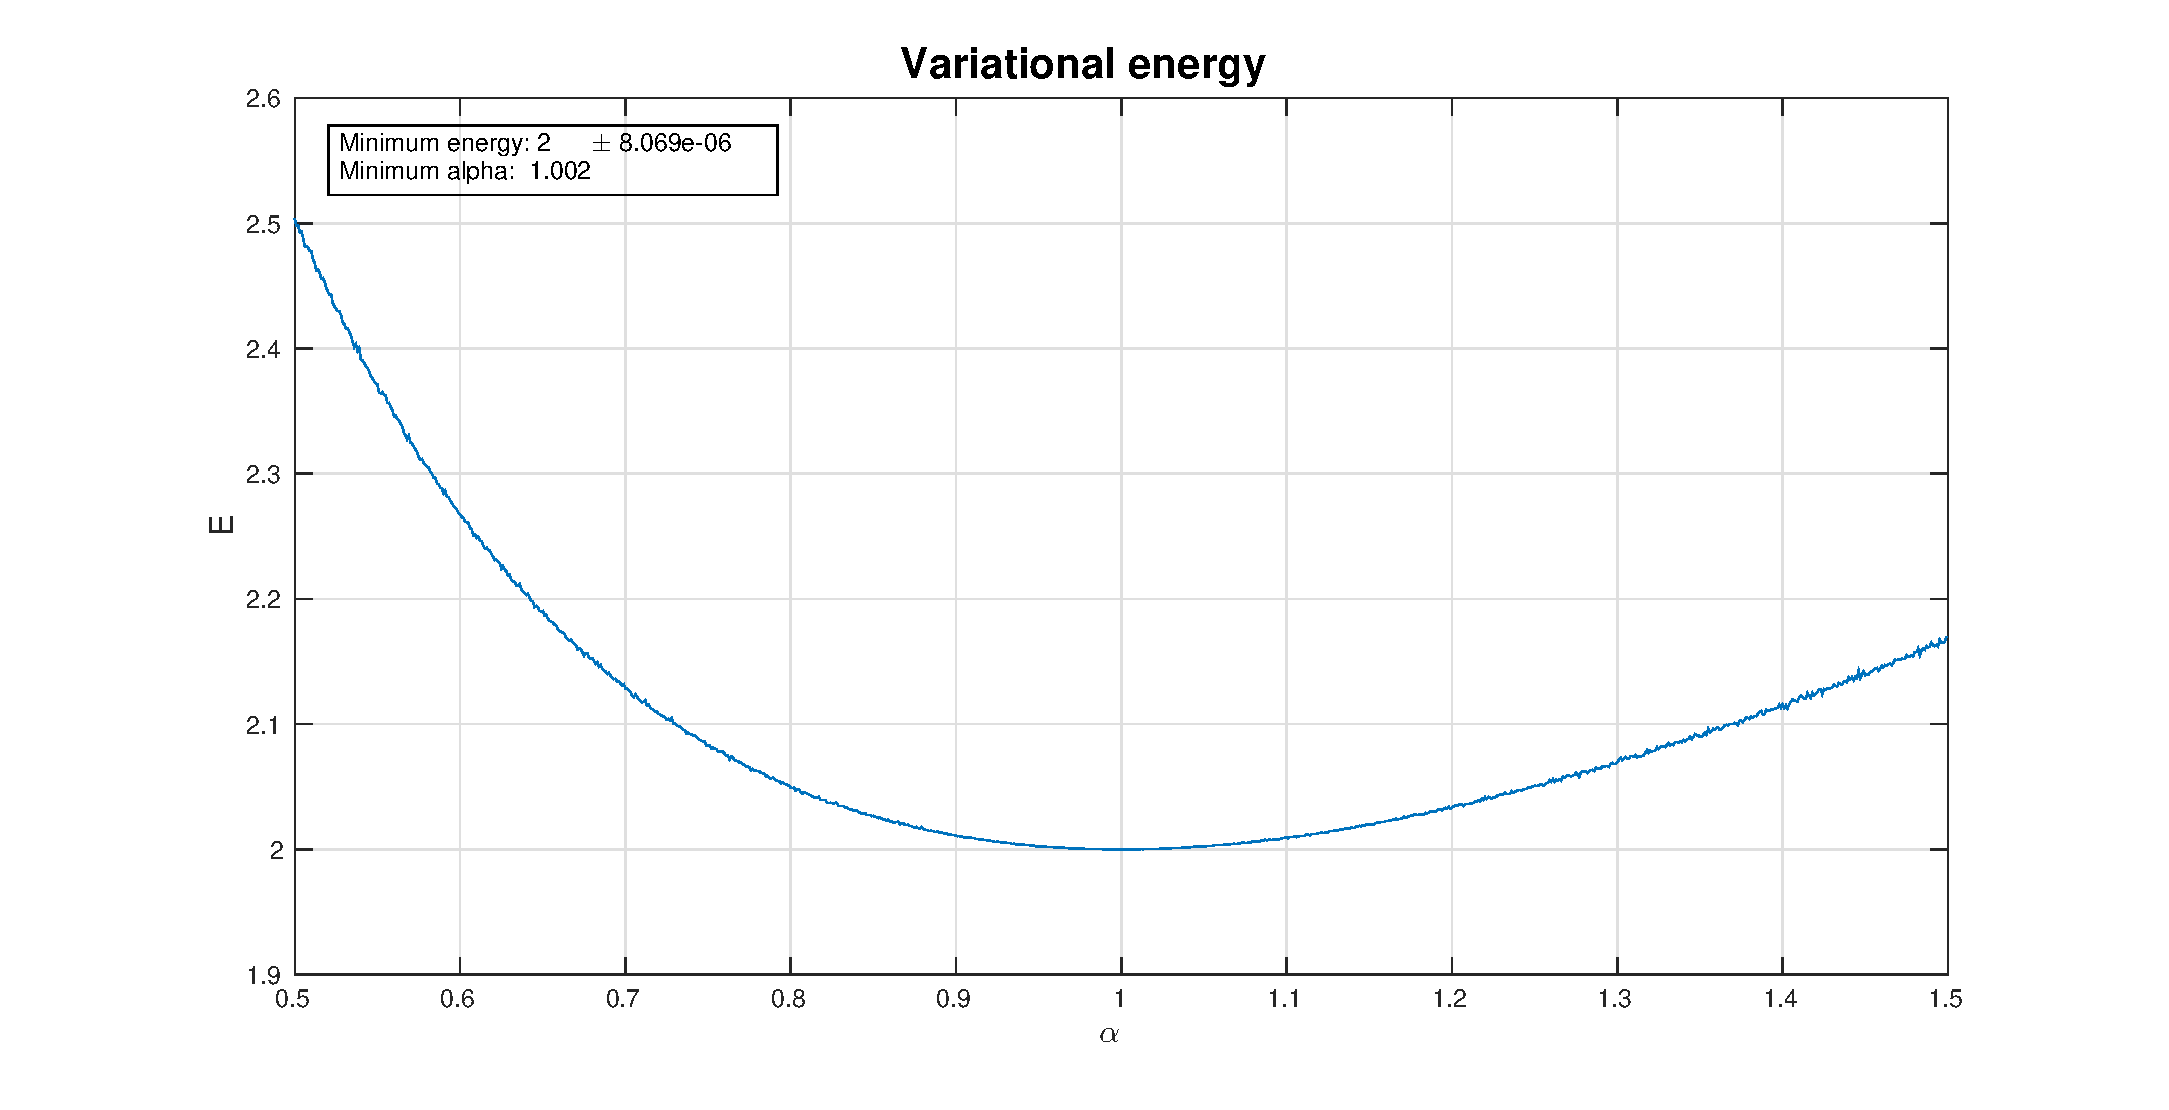
\includegraphics[width=\textwidth]{2e-norep}
	\caption{The variational energy versus the variational parameter $\alpha$. The settings used are: brute force sampling with step length 2, no Jastrow factor, no parallelization, $1000$ variations of $\alpha$ around $1$ with step $0.001$, $\SI{1e7}{}$ Monte Carlo steps. Acceptance ratio varies from $40$ to $\SI{60}{\percent}$.}
	\label{fig:2e_no_rep}
\end{figure}

As you can see in Figure \ref{fig:2e_no_rep}, we get $E_{\text{gs}} = 2$ with a high degree of precision for $\alpha=1$\footnote{Actually the minimum is for $\alpha=1.002$, but in this case we are not using so many steps that we can trust the third decimal digit. The smaller $\alpha$-step was just used to have a nicer plot.}.

We can also state that the total spin (better: its $z$-component) of the system is 0, as shown in equation (\ref{eq:total_spin}). If you want a more ``physical'' reason than just reading off a table of coefficients, this is a direct consequence of the shape of the wave-function for a fermionic system, as shown in equation (\ref{eq:slater_example}). In fact, in our case the spatial part of the two single-particle wave-functions is equal (they occupy the same energy level), yielding to
\begin{equation}
	\Ket{1} = \Ket{\phi}\otimes\Ket{\chi_1},
	\qquad
	\Ket{2} = \Ket{\phi}\otimes\Ket{\chi_2}.
\end{equation}
Comparing with equation (\ref{eq:identical_particles}) one sees that $\Ket{\psi} = 0$ unless $\Ket{1} \neq \Ket{2}$, and since the spatial parts are equal one has to conclude that $\Ket{\chi_1} \neq \Ket{\chi_2}$\footnote{We don't want $\Ket{\psi} = 0$ because it's not a physical state and it is not normalizable.}. Now, 
\begin{equation}
	\Ket{\chi_1} = \Ket{s,m_s}
\end{equation}
with $s=1/2$, so we have to say that -- for example -- particle 1 has spin-up ($m_s=1/2$) and particle 2 has spin-down ($m_s=-1/2$). This fact is also known as the \emph{Pauli exclusion principle}, and applies for a generic system of fermions.

\section{The complete system}
We want now to analyse the system with the full Hamiltonian, namely the Hamiltonian in equation (\ref{eq:full_hamiltonian}):
\begin{equation}
	\hat{H}=-\frac{1}{2} \nabla^2_1 - \frac{1}{2} \nabla^2_2+\frac{1}{2}\omega r_1^2+\frac{1}{2}\omega r_2^2+ \frac{1}{|\vec{r_1}-\vec{r_2}|},
\end{equation}
where $\vec{r_1}$ and $\vec{r_2}$ are the position operators of the two particles.

You see that this time we have a problem when two particles are very near to each other, since the term
\begin{equation*}
	\sum_{i<j}\frac{1}{|\vec{r_1}-\vec{r_2}|}
\end{equation*}
tends to be a division by zero. Introducing the substitution
\begin{equation}
\begin{cases}
\vec{r}=\vec{r_1}-\vec{r_2} \\ 
\vec{R}=\frac{1}{2}(\vec{r_1}+\vec{r_2}) 
\end{cases}
\end{equation}
the Hamiltonian can be rewritten in a decoupled way as \citep[see][]{Taut1993}
\begin{equation}
    \hat{H} = -\nabla_{\vec{r}}^2 - \frac{1}{4}\nabla_{\vec{R}}^2 - \frac{1}{4}\omega^2\vec{r}^2 + \omega^2\vec{R}^2 + \frac{1}{r}.
\end{equation}
Since the Hamiltonian is spin-independent, we can factorize the wave-function as
\begin{equation}
    \psi(\vec{r},\vec{R},m_{s_1},m_{s_2}) = \varphi(\vec{r})\xi(\vec{R})\chi(m_{s_1},m_{s_2})
\end{equation}
which separates the Schr\"{o}dinger equation into
\begin{equation}
    \left( -\frac{1}{2}\nabla_{\vec{r}}^2 + \frac{1}{2}\omega_r^2\vec{r}^2 + \frac{1}{2}\frac{1}{r} \right)\varphi(\vec{r}) = E_r\varphi(\vec{r})
    \label{eq:Seq_relative_distance}
\end{equation}
and
\begin{equation}
    \left( -\frac{1}{2}\nabla_{\vec{R}}^2 + \frac{1}{2}\omega_R^2\vec{R}^2 \right)\xi(\vec{R}) = E_R\xi(\vec{R}),
\end{equation}
where $\omega_r = \frac{1}{2}\omega$ and $\omega_R = 2\omega$.

We are not interested in the $R$-part of the solution, since it gives no troubles; we are more interested in equation \eqref{eq:Seq_relative_distance}, because we can cancel the divergence for $r \to 0$ working on the solution. We can also forget about the harmonic potential because it gives no divergence. Since we are only interested in the radial part of the solution, the relevant contributions from the laplacian in spherical coordinates are
\begin{equation}
    \nabla^2_r = \frac{d^2}{dr^2} + \frac{1}{r}\frac{d}{dr}.
\end{equation}
We also notice that $\frac{d^2}{dr^2}$ gives a finite contribution (is just the momentum part) and so does $\frac{d}{dr}$. The only piece that is not finite is the $\frac{1}{r}$ in front of $\frac{d}{dr}$, that we can use to cancel the divergence in the interaction potential. Using these facts, equation \eqref{eq:Seq_relative_distance} can be rewritten in a way that is called the \emph{cusp condition} for this system, namely
\begin{equation}
    \lim_{r \to 0} \frac{1}{\varphi(r)}\left( -\cancel{\frac{1}{2}\frac{1}{r}}\frac{d}{dr} + \cancel{\frac{1}{2}\frac{1}{r}} \right)\varphi(r) = 0.
\end{equation}
Solving for $\varphi$ by partial integration gives
\begin{equation}
    \varphi(r) = \exp(Cr),
    \qquad\qquad
    r \to 0
    \label{eq:cusp_solution}
\end{equation}
where $C$ is a constant. For these types of Monte Carlo calculations, a so-called \emph{Padé-Jastrow} factor that has the property \eqref{eq:cusp_solution} is often used. This factor has the form (for two electrons)
\begin{equation}
    \exp\left( \frac{ar}{(1+\beta r)} \right),
\end{equation}
where (in 2 dimensions)
\begin{equation}
    a = 
    \begin{cases}
    1 & \text{anti-parallel spin} \\
    1/3 & \text{parallel spin}
    \end{cases}
\end{equation}
and $\beta$ is a variational parameter. With this factor, our trial wave-function reads as
\begin{equation}
    \psi_T(\vec{r_1},\vec{r_2}) = \exp\left(-\alpha\omega\left(r_1^2 + r_2^2\right)/2\right)\exp\left( \frac{ar}{(1+\beta r)} \right).
    \label{eq:wf_2e}
\end{equation}

Using the ansatz in equation \eqref{eq:wf_2e} in our program, we obtain a preliminary result shown in Figure \ref{fig:2e_rep}.

\begin{figure}[h]%[H]
	\centering
	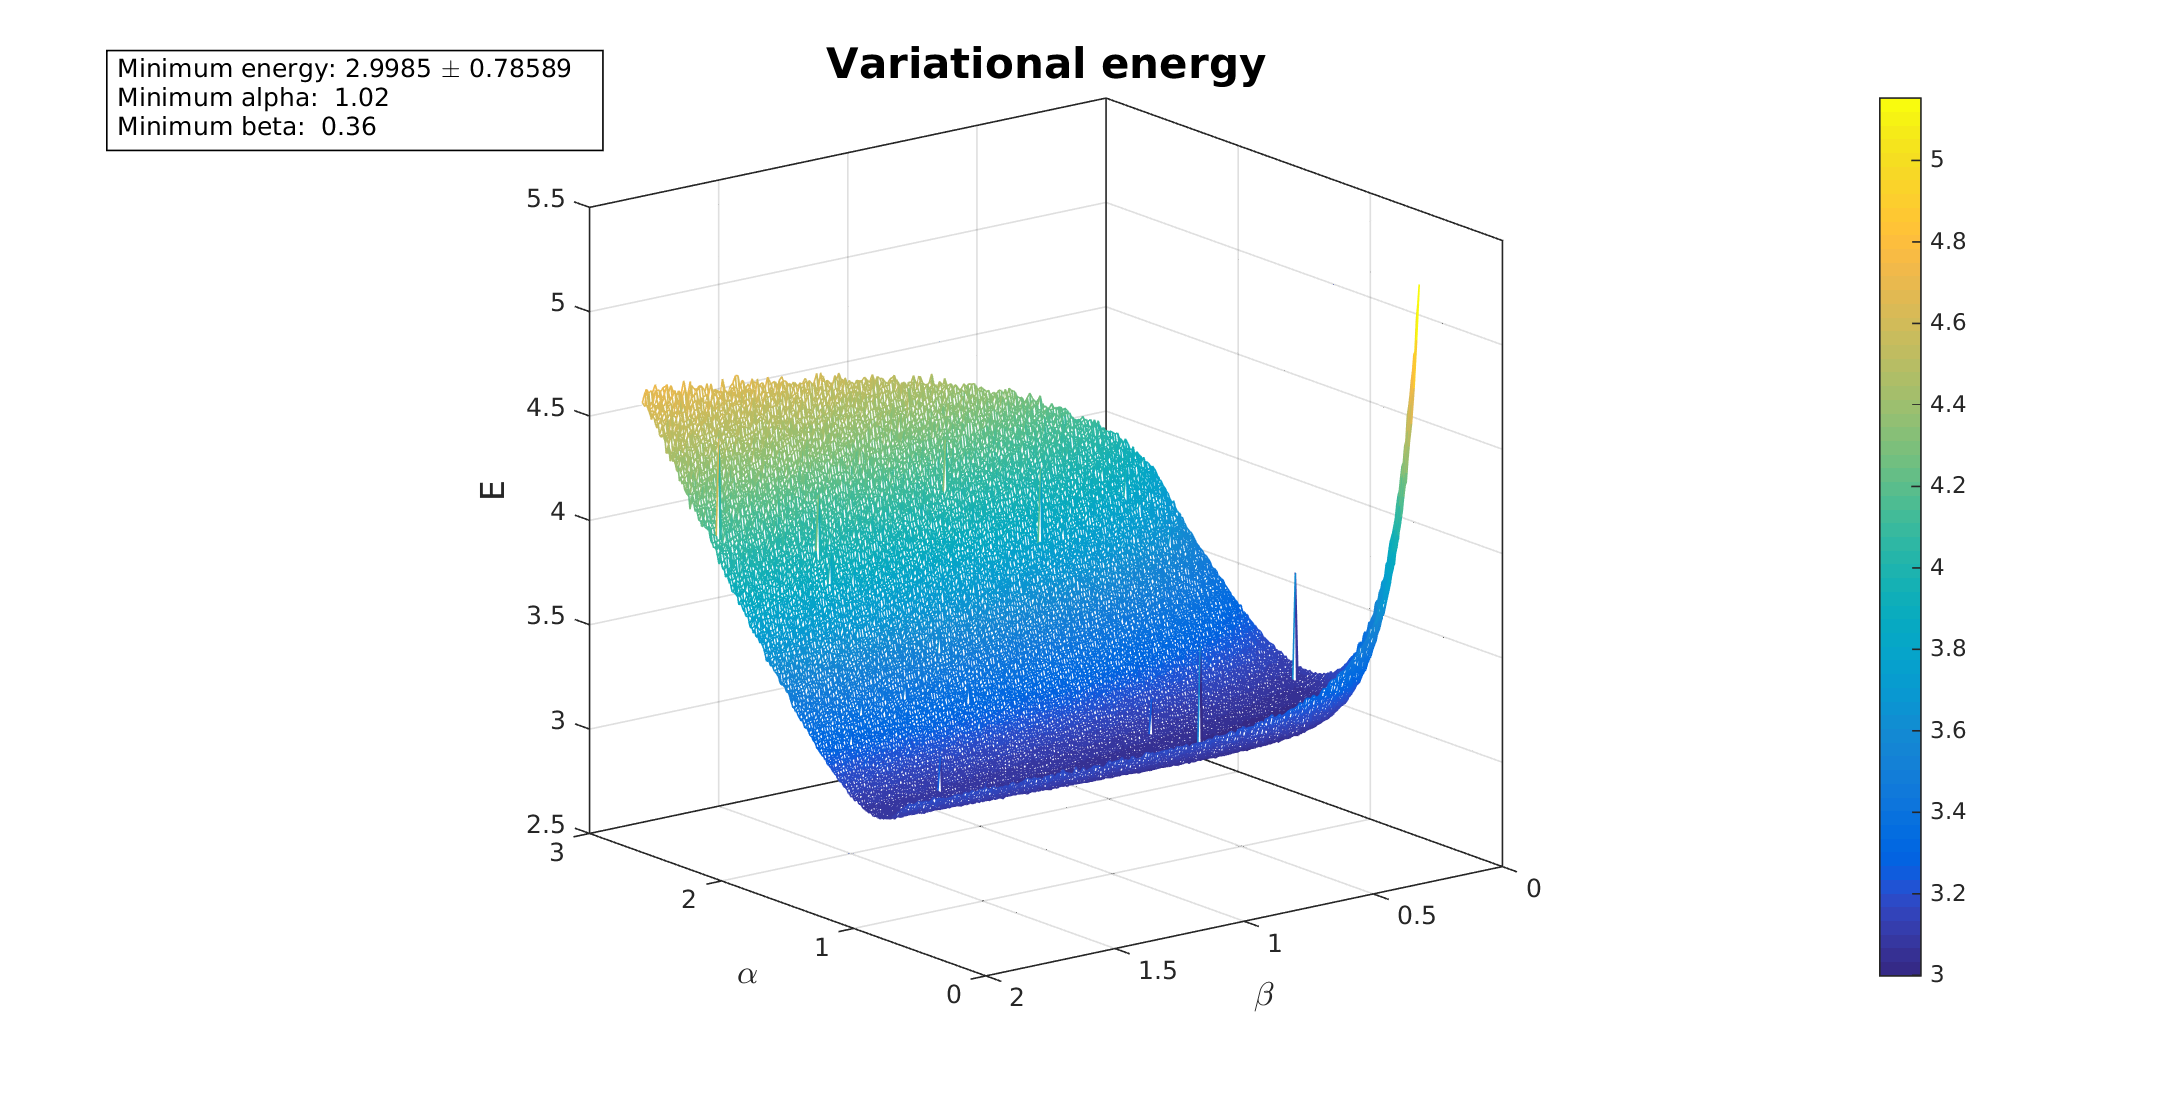
\includegraphics[width=\textwidth]{2e-rep}
	\caption{The variational energy versus the variational parameters $\alpha$ and $\beta$. The settings used are: brute force sampling with step length 2, Jastrow factor, no parallelization, $200$ variations of $\alpha$ and $\beta$ with step $0.01$, $\SI{1e5}{}$ Monte Carlo steps. Acceptance ratio varies from $45$ to $\SI{55}{\percent}$.}
	\label{fig:2e_rep}
\end{figure}

Refining around the minimum value to have better results, we finally obtain the plot in Figure \ref{fig:2e_rep_fine}.

You see that we are very near to the exact result $E_{\text{gs}} = \SI{3}{\atomicunit}$ calculated from \cite{Taut1993} and reported in \cite{PedersenLohne2011}. However, the energy error is still quite big; a way to improve the precision of our program is to \emph{parallelize} it.

\begin{figure}[H]
	\centering
	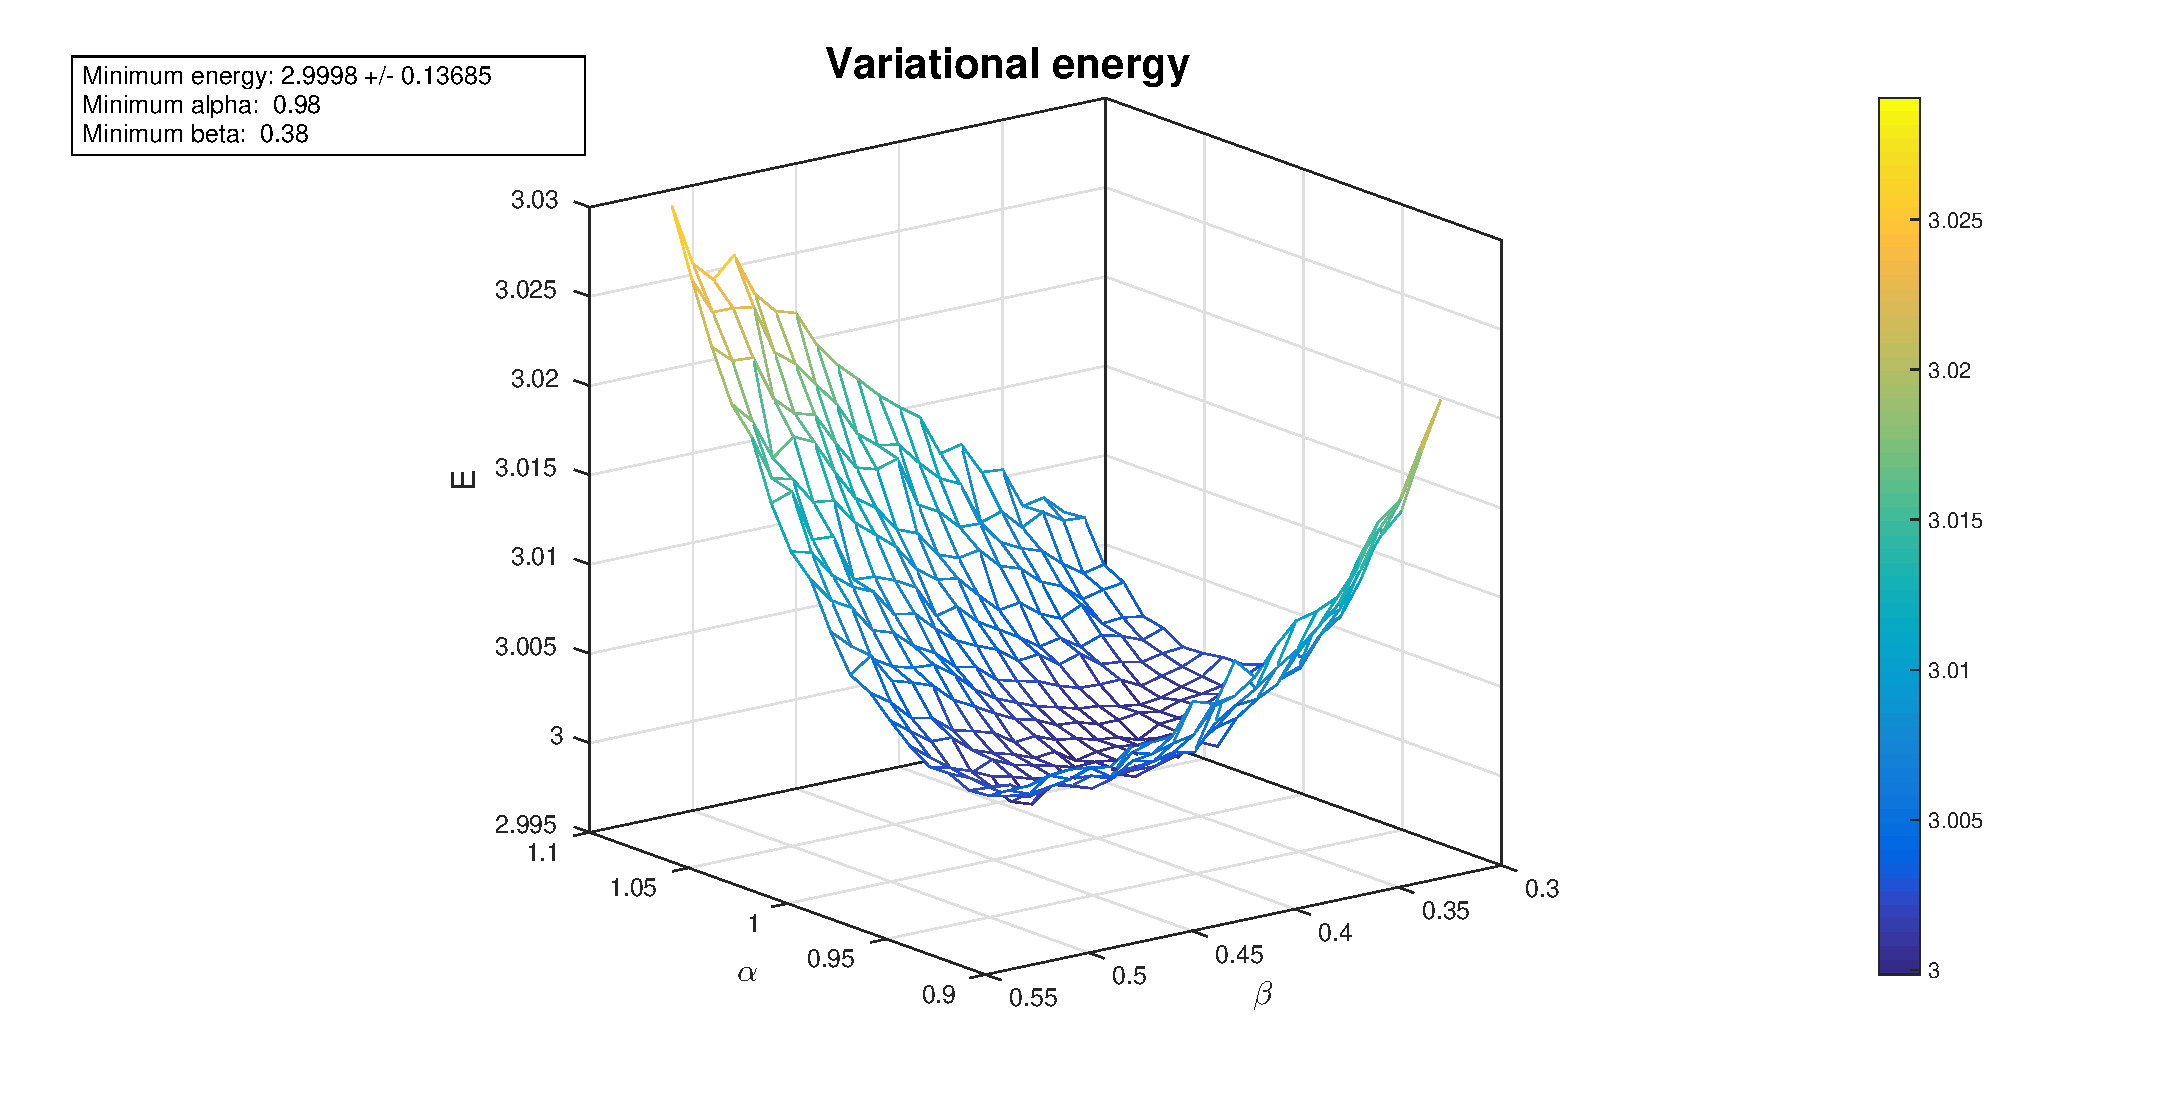
\includegraphics[width=\textwidth]{2e-rep_fine}
	\caption{The variational energy versus the variational parameters $\alpha$ and $\beta$. The settings used are: brute force sampling with step length 2, Jastrow factor, no parallelization, $20$ variations of $\alpha$ and $\beta$ with step $0.01$, $\SI{1e6}{}$ Monte Carlo steps. Acceptance ratio varies from $45$ to $\SI{55}{\percent}$. The relative distance is about $\SI{1.64}{}$ in natural units.}
	\label{fig:2e_rep_fine}
\end{figure}

\subsection{Parallelization}

In this project, parallelization is done by using OpenMP\footnote{\url{http://openmp.org/}.}. The main idea is to run multiple computations of $E_T$ for the same pair of variational parameters $(\alpha,\beta)$ and then take the mean. Since the ``measurements'' of $E_T$ are not correlated, the error on its mean value falls like $1/\sqrt{n}$, where $n$ is the number of measurements. To be sure that the measurements are not correlated we have to make \emph{private} local copies of the variables used in the computation, one for each thread used. Then, we have to sync all the threads in order to be sure that all the measurements are complete, and finally we can take the mean. An example of how this is implemented in our program is given below:

\begin{lstlisting}[language=cpp]
    // Begin parallelization
    omp_set_num_threads(gP.num_threads);
    #pragma omp parallel shared(cumulative_e, cumulative_e2)
    {
        // Make a private copy of all the stuff
        mat cumulative_e_local = zeros<mat>(vmcParams.max_variations+1,vmcParams.max_variations+1);
        mat cumulative_e2_local = zeros<mat>(vmcParams.max_variations+1,vmcParams.max_variations+1);
        struct GeneralParams gP_local = gP;
        struct VariationalParams vP_local = vP;
        struct VMCparams vmcParams_local = vmcParams;

        // Build the orbitals
        Orbitals* MyWaveFunction_local = new AlphaHarmonicOscillator(gP_local, vP_local);

        // Set up the Jastrow factor
        Jastrow* MyJastrowFactor_local;
        if (vmcParams_local.jF_active) MyJastrowFactor_local = new Pade_Jastrow(gP,vP);
        else MyJastrowFactor_local = new No_Jastrow();

        // Make a local copy of the system for convenience
        System MySystem_local = MySystem;

        // Do the mc sampling
        mc_sampling(gP_local, vP_local, vmcParams_local,
                    cumulative_e_local, cumulative_e2_local,
                    MySystem_local, MyWaveFunction_local, MyJastrowFactor_local);

        // Be sure to have all the contributions
        #pragma omp barrier
        #pragma omp critical
        {
            // Add the contributions
            cumulative_e += cumulative_e_local;
            cumulative_e2 += cumulative_e2_local;
        }
    }

    // Normalize to the number of threads
    cumulative_e = cumulative_e/((double) gP.num_threads);
    cumulative_e2 = cumulative_e2/((double) gP.num_threads);
\end{lstlisting}

Re-doing the calculations using parallelization gives the result in Figure \ref{fig:2e_rep_parallel}.
\begin{figure}[H]
	\centering
	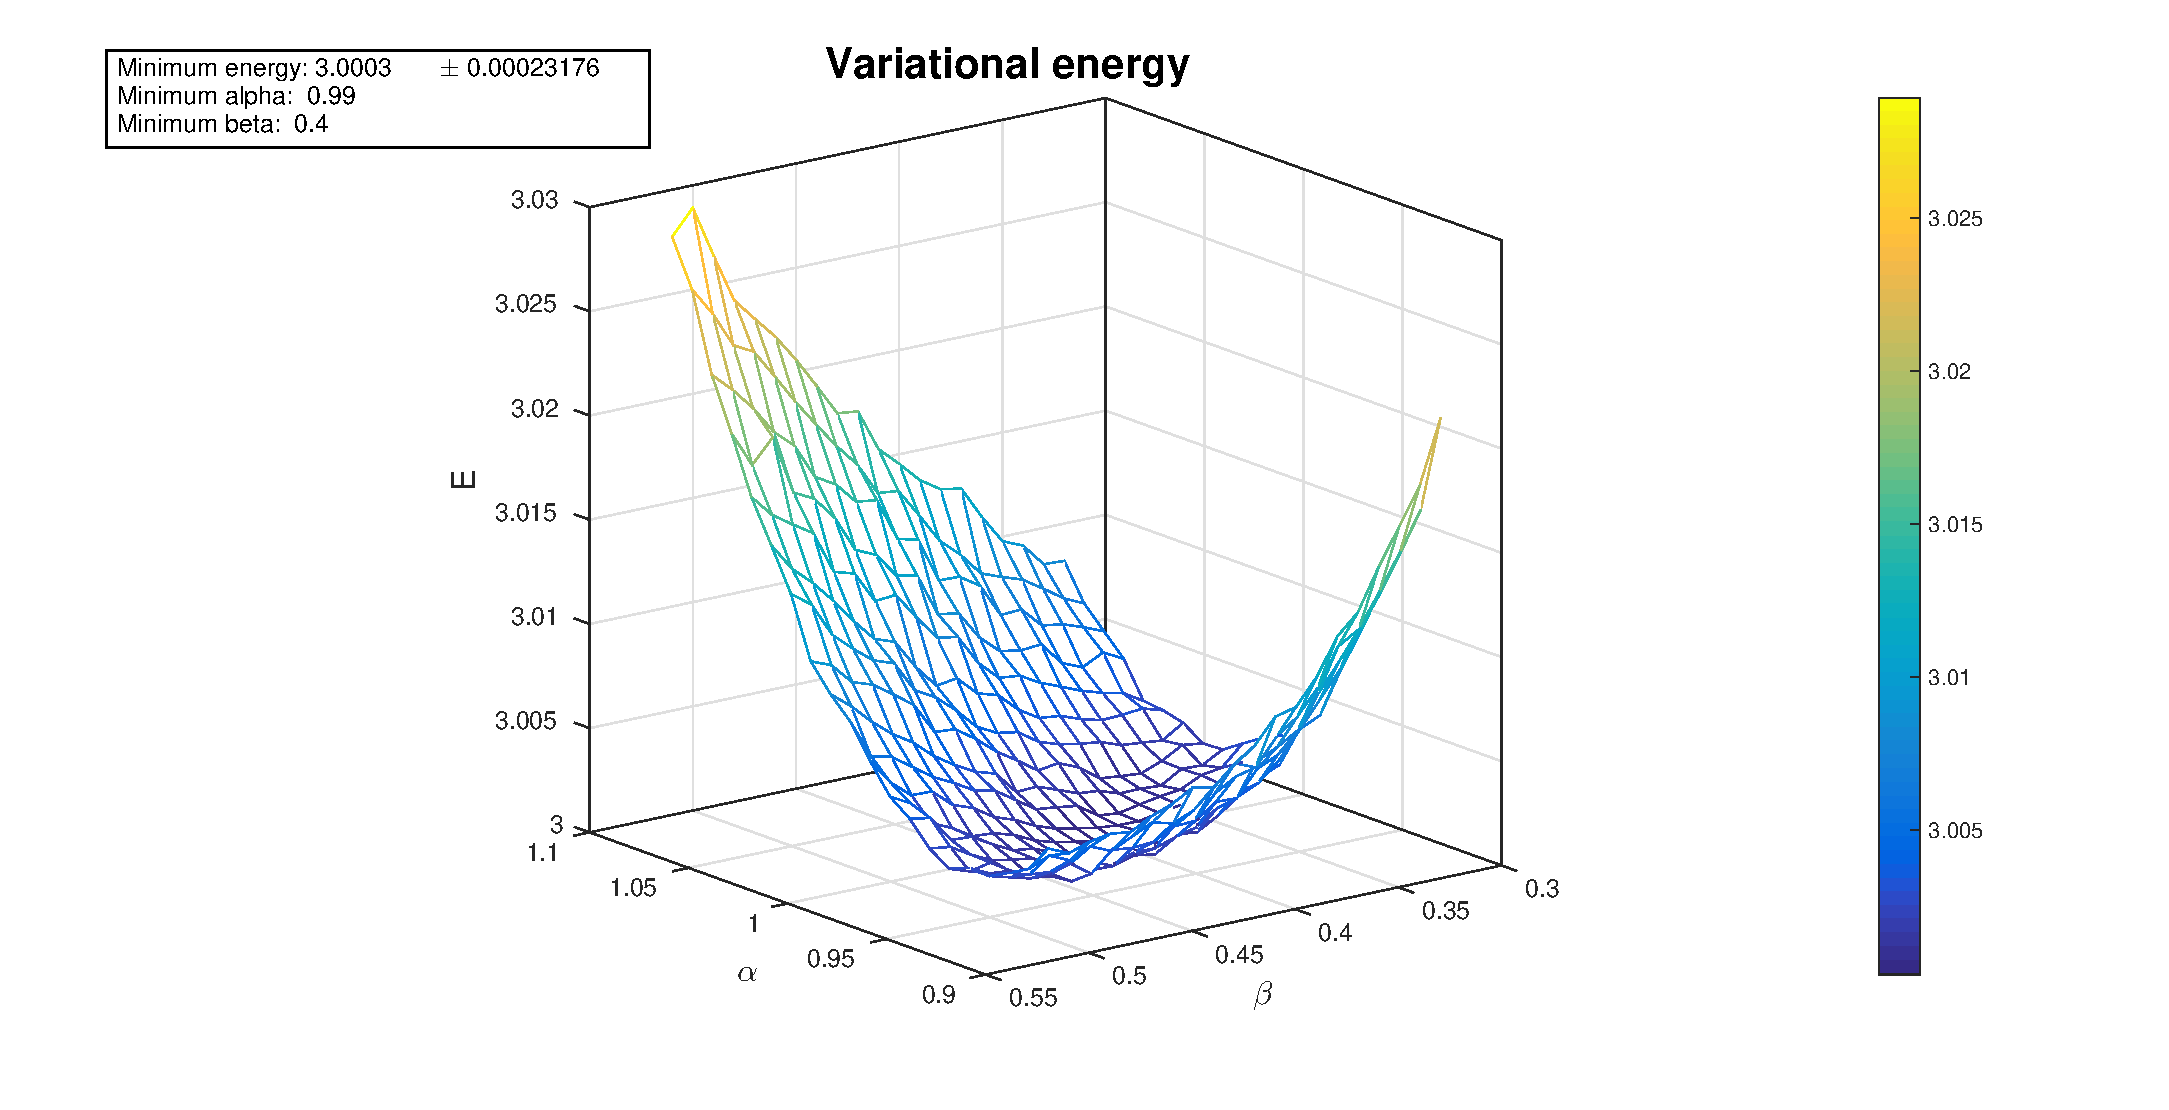
\includegraphics[width=\textwidth]{2e-rep_parallel}
	\caption{The variational energy versus the variational parameters $\alpha$ and $\beta$. The settings used are: brute force sampling with step length 2, Jastrow factor, parallelization (8 threads), $20$ variations of $\alpha$ and $\beta$ with step $0.01$, $\SI{2e5}{}$ Monte Carlo steps. Acceptance ratio varies from $45$ to $\SI{55}{\percent}$.}
	\label{fig:2e_rep_parallel}
\end{figure}
Note that this time, even using a lower number of Monte Carlo steps, we have an amazingly precise estimate for our energy, comparable with the one obtained in \cite{PedersenLohne2011} using Diffusion Monte Carlo.

\subsection{Importance sampling}
Let's now try to implement importance sampling, as explained in Section \ref{sec:importance}. In order to show the differences with the brute force algorithm, we will repeat the calculations with exactly the same settings used in Figure \ref{fig:2e_rep_parallel}, this time with importance sampling active. We will also try to do the calculations for different time-steps $\Delta t = 0.001,\,0.01,\,0.1$.

The results are shown in Figures \ref{fig:2e-rep_imp_small}, \ref{fig:2e-rep_imp_med} and \ref{fig:2e-rep_imp_high}.

As you see, there is a huge difference between the result obtained with $\Delta t = 0.001$ and the one obtained with $\Delta t = 0.1$. This is because, if the time step is too small and we don't have enough Monte Carlo steps, our walker cannot span completely the integration space. It will remain near its starting point and all the points reached will be inside the integration space, close to each other. In fact, the acceptance ratio for the case $\Delta t = 0.001$ and $\Delta t = 0.01$ is \emph{practically} $\SI{100}{\percent}$. The third case, for $\Delta t = 0.1$, has a little lower acceptance ratio, that is about $\SI{99.79}{\percent}$. This fact guarantees that our walker is reaching all the borders of our integration space, and in fact it also reaches some points outside it. In other words, for the given number of Monte Carlo iterations, we have a time-step large enough to cover all the space. If one wants to use a lower time-step to have better precision, he has to increase the number of Monte Carlo cycles; as an example, for $\Delta t = 0.001$, one has to use at least $\SI{1e9}{}$ Monte Carlo loops.

\begin{figure}[H]
	\centering
	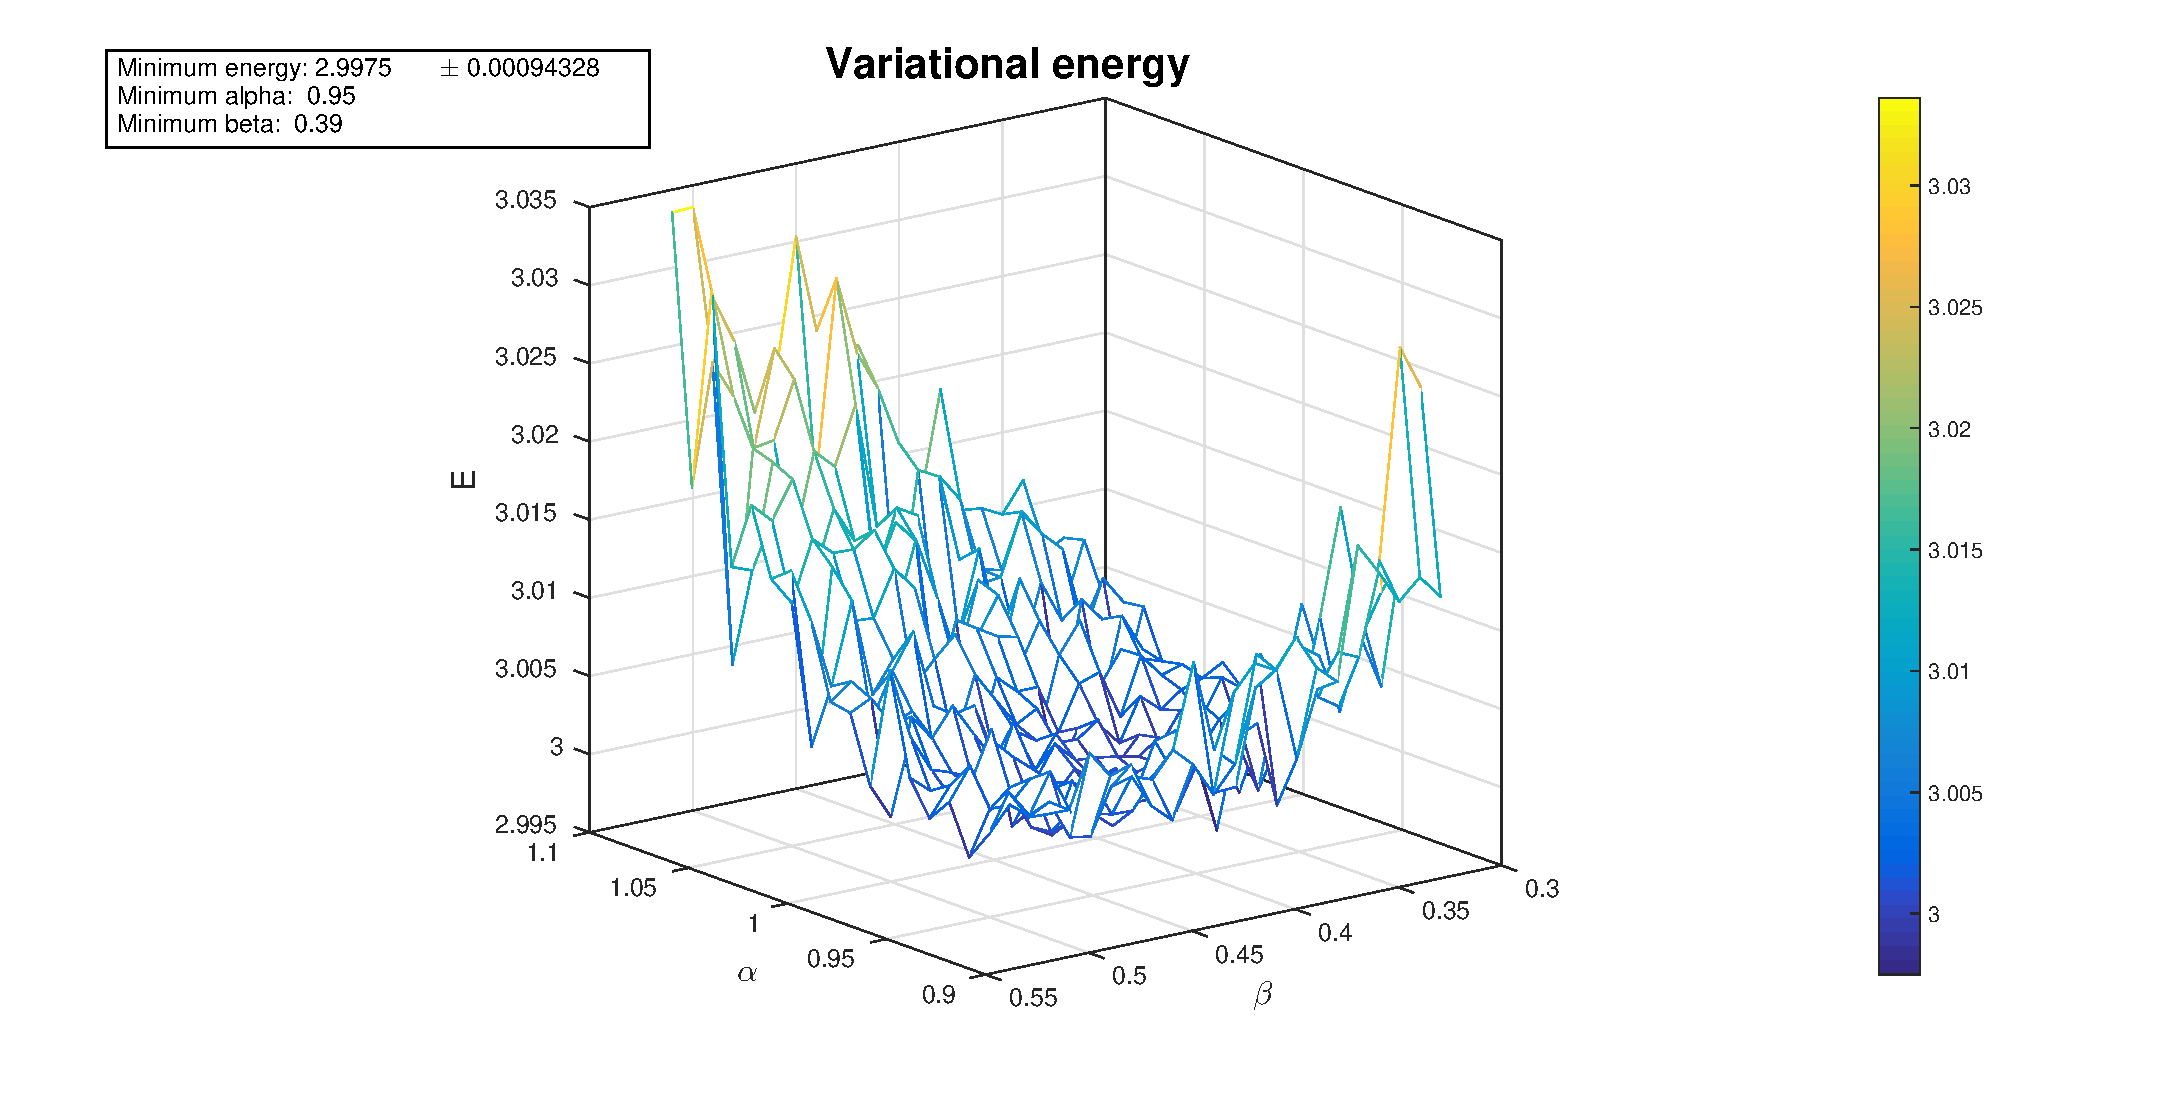
\includegraphics[width=\textwidth]{2e-rep_imp_small}
	\caption{The variational energy versus the variational parameters $\alpha$ and $\beta$. The settings used are: importance sampling with $\Delta t = 0.001$, Jastrow factor, parallelization (8 threads), $20$ variations of $\alpha$ and $\beta$ with step $0.01$, $\SI{2e5}{}$ Monte Carlo steps. Acceptance ratio is about $\SI{99.999}{\percent}$.}
	\label{fig:2e-rep_imp_small}
\end{figure}
\begin{figure}[H]
	\centering
	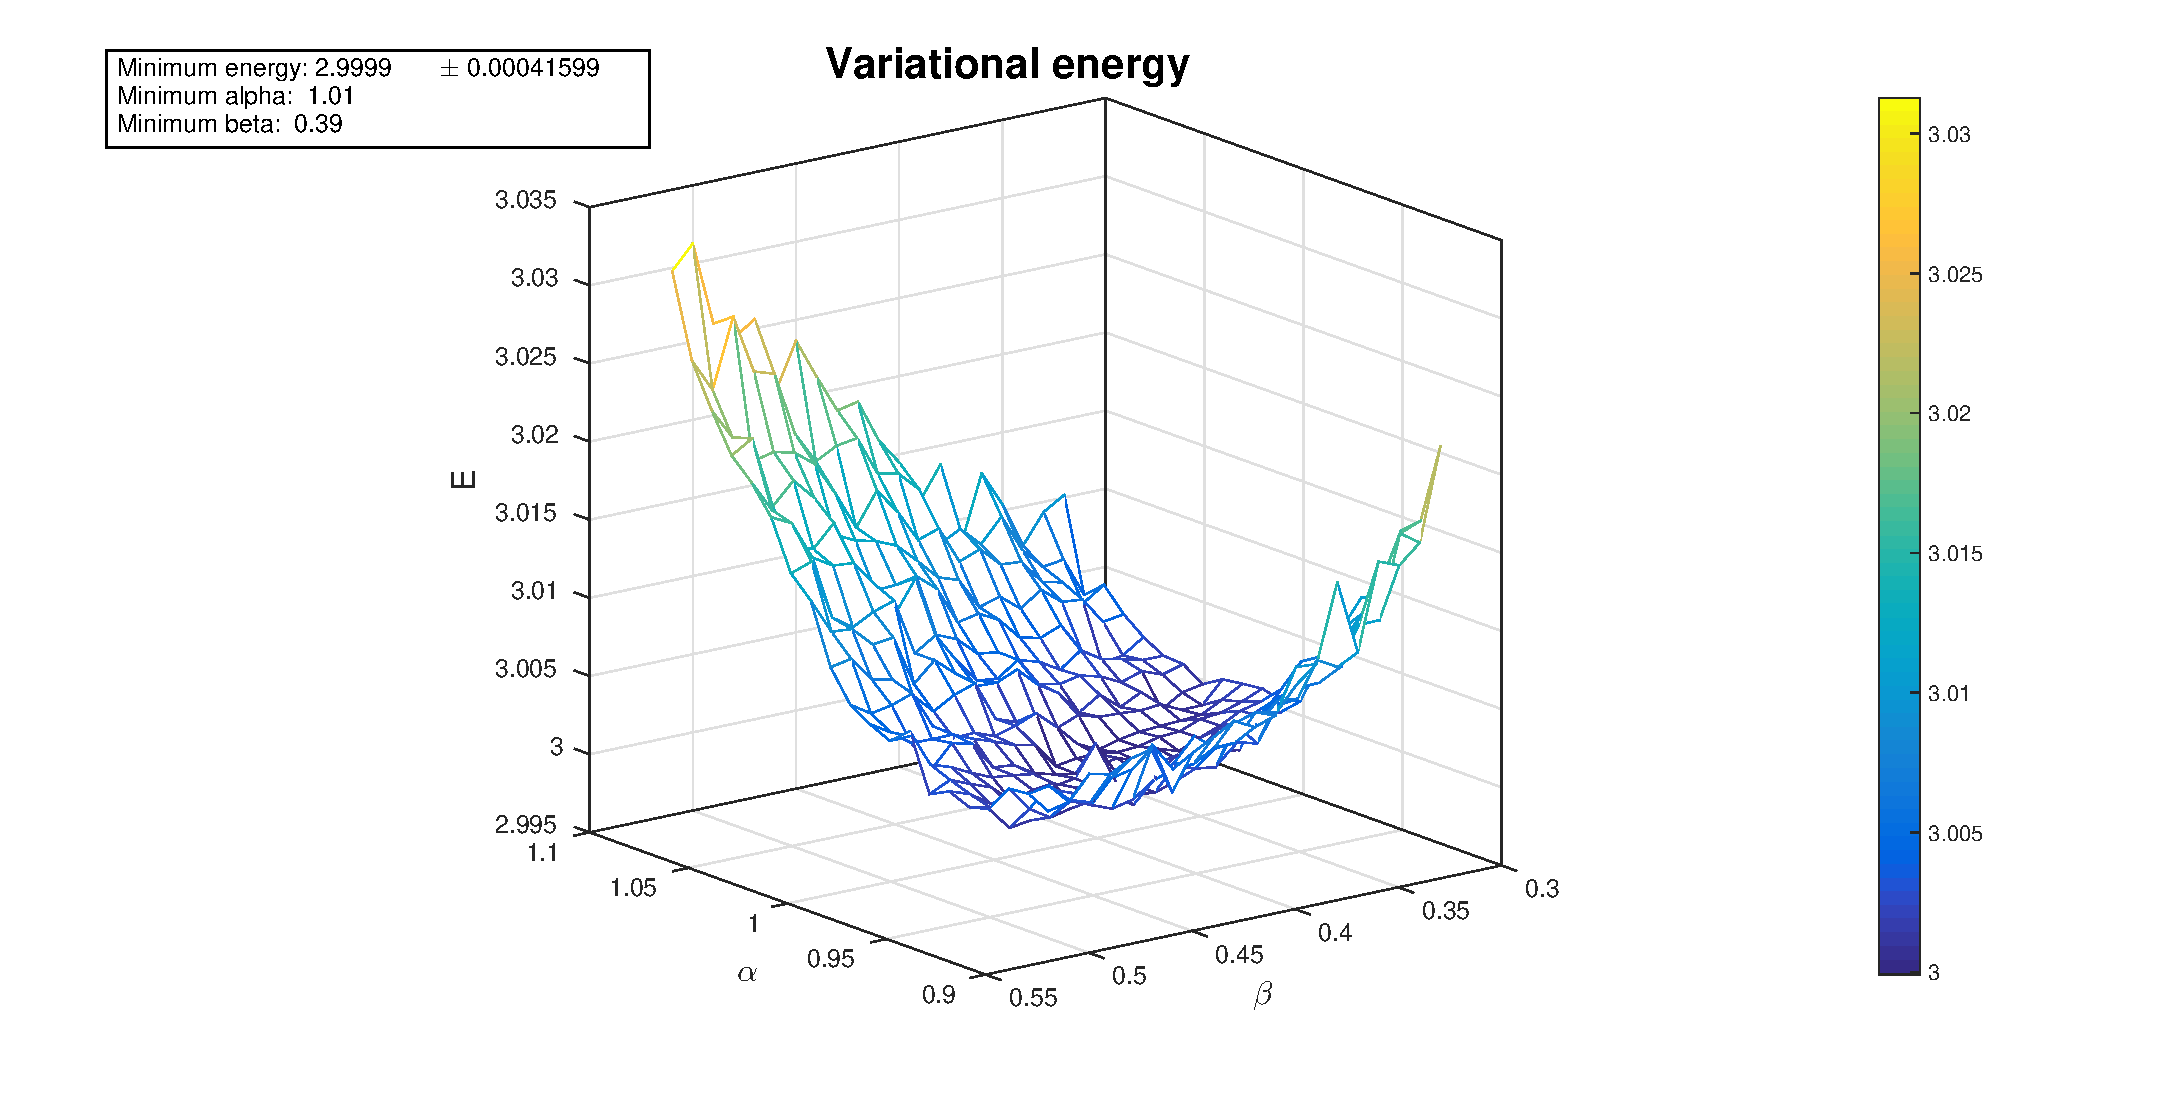
\includegraphics[width=\textwidth]{2e-rep_imp_med}
	\caption{The variational energy versus the variational parameters $\alpha$ and $\beta$. The settings used are: importance sampling with $\Delta t = 0.01$, Jastrow factor, parallelization (8 threads), $20$ variations of $\alpha$ and $\beta$ with step $0.01$, $\SI{2e5}{}$ Monte Carlo steps. Acceptance ratio is about $\SI{99.999}{\percent}$.}
	\label{fig:2e-rep_imp_med}
\end{figure}
\begin{figure}[H]
	\centering
	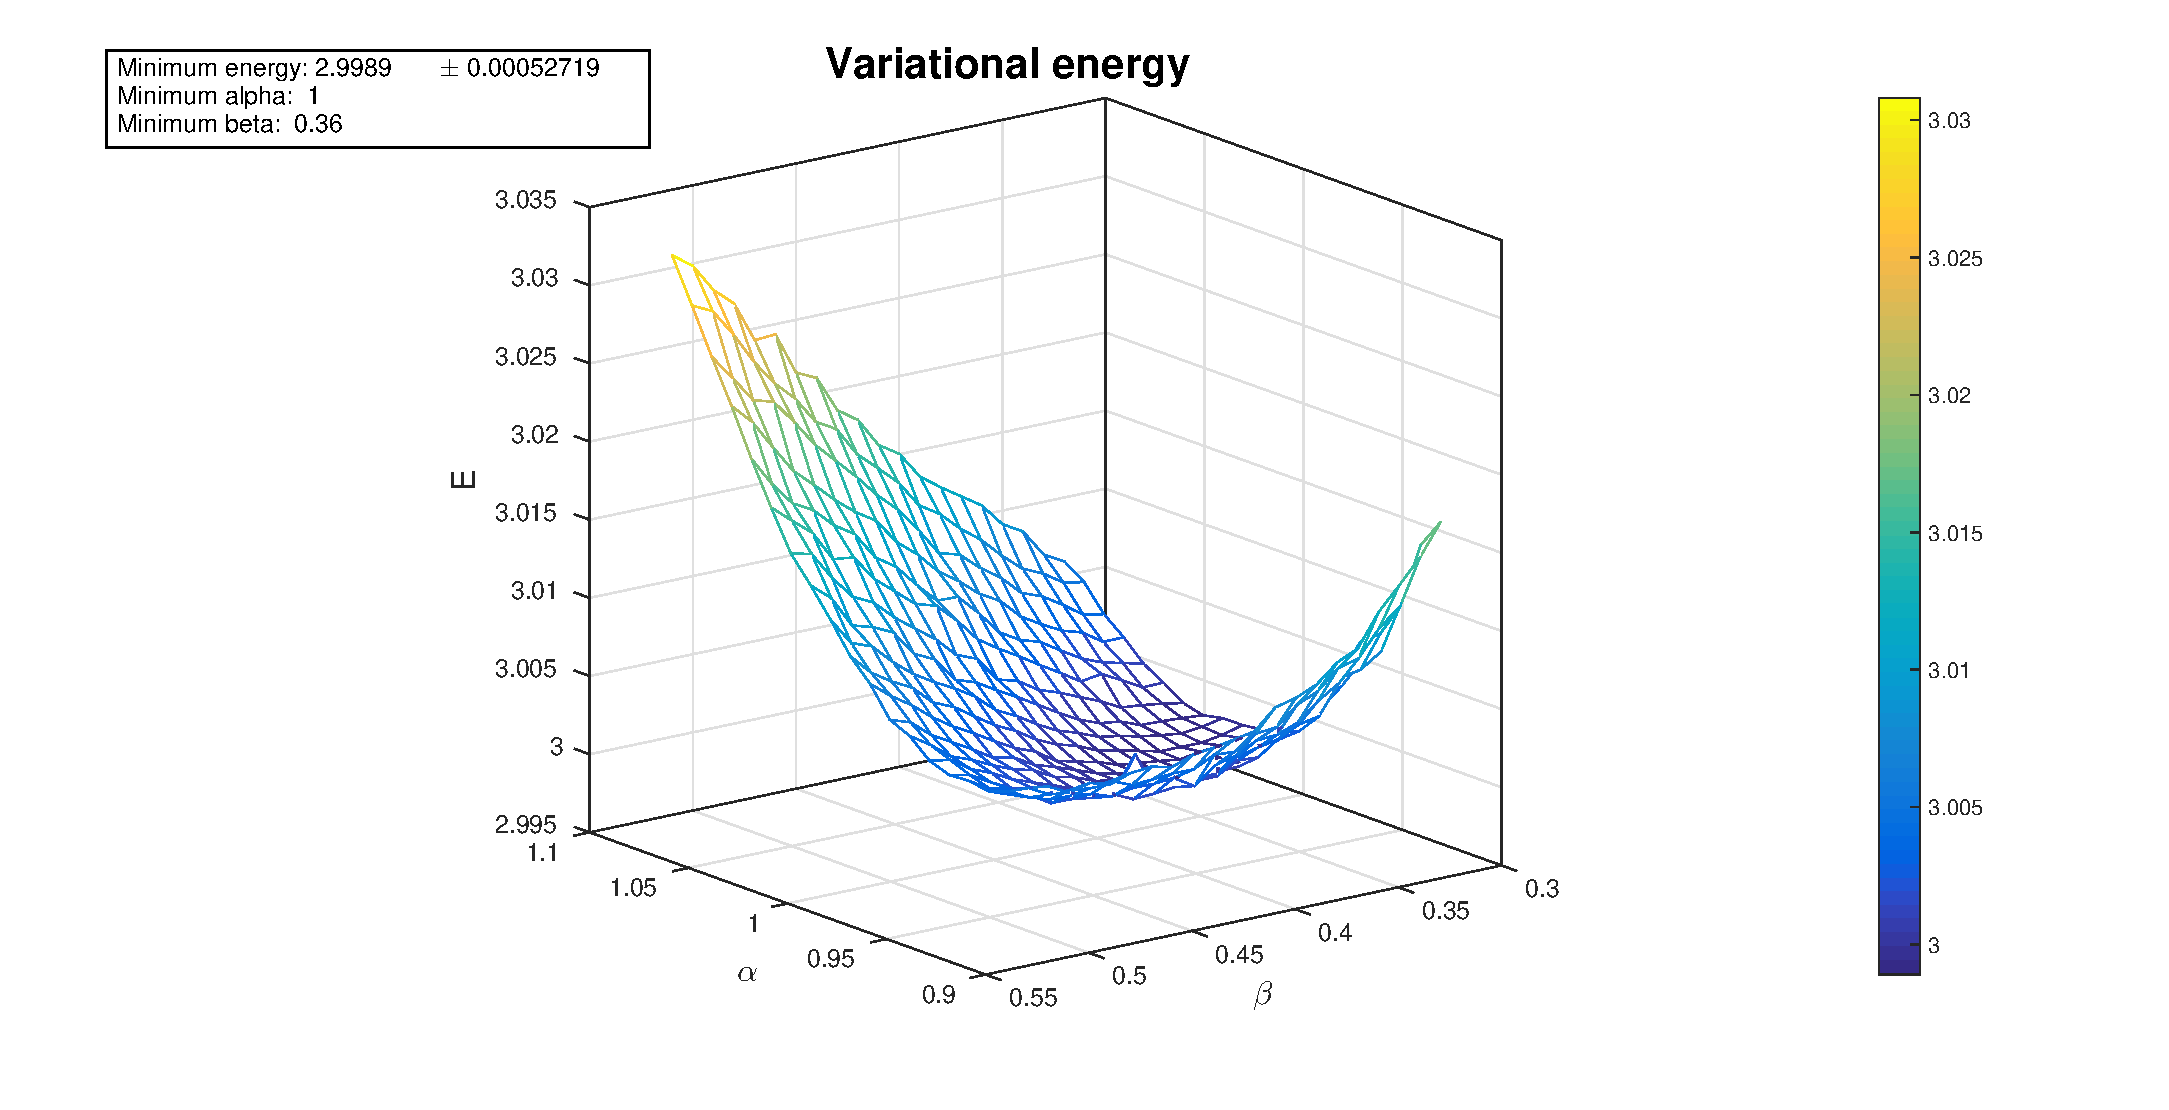
\includegraphics[width=\textwidth]{2e-rep_imp_high}
	\caption{The variational energy versus the variational parameters $\alpha$ and $\beta$. The settings used are: importance sampling with $\Delta t = 0.1$, Jastrow factor, parallelization (8 threads), $20$ variations of $\alpha$ and $\beta$ with step $0.01$, $\SI{2e5}{}$ Monte Carlo steps. Acceptance ratio is about $\SI{99.793}{\percent}$.}
	\label{fig:2e-rep_imp_high}
\end{figure}